% !TeX root = RJwrapper.tex
\title{The \CRANpkg{crossrun} package: Joint Distribution for Number of Crossings and Longest Run in Independent Bernoulli observations}
\author{by Tore Wentzel-Larsen and Jacob Anh{\o}j}

\maketitle

\abstract{
The package \CRANpkg{crossrun} computes the joint distribution of the number of crossings and the longest run in a sequence of independent Bernoulli observations. The main intended application is statistical process control where the joint distribution may be used for systematic investigation, and possibly refinement, of existing rules for distinguishing between signal and noise. While the \CRANpkg{crossrun} vignette is written to assist in practical use, this article gives a hands-on explanation of \emph{why} the procedures works. The article also includes a discussion of limitations of the present version of \CRANpkg{crossrun} together with an outline of ongoing work to meet these limitations. There is more to come, and it is necessary to grasp the basic ideas behind the procedure implemented both to understand these planned extensions, and how presently implemented rules in statistical process control, based on the number of crossings and the longest run, may be refined.
}

\section{Introduction}

The setting is defined by a number of independent observations from a Bernoulli distribution with the same success probability. In statistical process control, our main intended application, this may be the useful observations in a runchart, recording values above and below the median from previous data, disregarding any observations equal to the median \citep{Anhoej:2015}. 

The focus of the \CRANpkg{crossrun} package is the joint distribution of number of crossings, $C$, and the length of the longest run, $L$, in random data sequences. A run is a sequence of successes or failures, delimited by a different observation or the start or end of the entire sequence. A crossing is two adjacent different observations. 

Figure~\ref{figure:fig1} illustrates runs and crossings in a run chart with 20 random observations. Observations above and below the median represent successes and failures respectively.

\begin{figure}[htbp]
  \centering
  \caption{A runchart with $n=20$ data points. The longest run consists of observations 3-7 above the median. The length of the longest run is $L=5$. The number of crossings of the median is $C=10$.}
  \label{figure:fig1}
  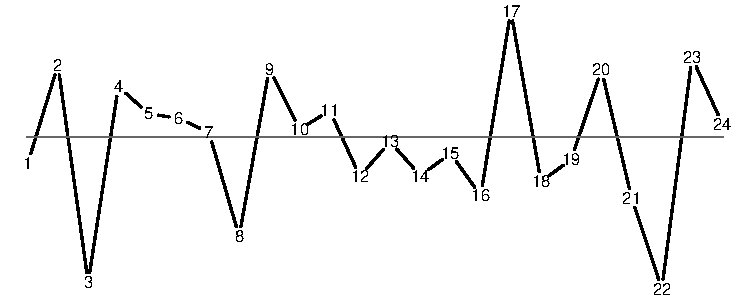
\includegraphics[width=0.95\textwidth]{fig1}
\end{figure}

While the number of crossings follows a binomial distribution in the symmetric case (success probability 0.5), no closed form distribution is known for the longest run. The distribution of the longest run has been investigated in a number of articles, including \citep{Schilling:2012}, and \citep{Fazekas:2010} that in fact gives recursion formulas, and approximations have been given. However, what is needed in applications is the joint distribution of these two variables, for which we are not aware of exact results. Our primary aim is to present an iterative procedure for computing this distribution, in principle for an arbitrary number of observations.

\section{The iterative procedure, setting}

In $n$ independent Bernoulli observations with success probability $p$ and failure probability $q = 1 - p$, values are denoted by 1 (success with probability $p$) or 0. A crossing consists of two consecutive different values, and a run of length $l$ consists of $l$ successive observations, delimited by a crossing or the first or last observation. The possible values of the number $C$ of crossings are $c=0, \ldots ,n-1$ and the possible values for the length $L$ of the longest run are $l=1, \ldots ,n$. The joint probabilities of $L$ and $C$ for given $n$ are denoted by $P_n (L=l,C=c)$.

The iterative procedure involves conditioning on the first observation denoted by $S$, with values 1 for success (probability $p$) and 0 for failure (probability $q$). The iterative procedure computes the conditional probabilities 

$$P_n (L=l,C=c \mid S=1), P_n (L=l,C=c \mid S=0)$$

This conditioning on the first observation is an essential part of the procedure. One way to see that this is reasonable is to consider the case when $p$ is close to 1. Then most observations are successes, most runs are success runs and the conditional joint distribution of runs and crossings is quite different dependent on the first observation. It is sufficient to be able to compute these conditional distributions, because the unconditional joint distribution is $$P_n (L=l,C=c) = P_n (L=l,C=c \mid S=1) \cdot p + P_n (L=l,C=c \mid S=0) \cdot q$$ For the iterative procedure to work it is also necessary to take another variable into account, the first crossing. More precisely, we denote the end position of the first crossing by $F$, with values $f=2, \ldots ,n$. An additional value $f=1$ denotes, by convention, the case of no crossing. The joint probabilities for $C$ and $L$ conditional on $S$ are partioned by further conditioning on $F$ as detailed below.

It is important to underline that the conditioning variables $S$ and $F$ are not parameters of the distribution but useful constructions that help break down the iterative procedure in manageable parts.

This article first describes the setting for the iterative computation procedure and its initial stage. Next we introduce conditioning on the starting position and partitioning on the position of the first crossing. Finally, the joint distribution of the number of crossings and the longest run conditional on these variables is given. The computation procedure is different in two cases that are subsequently described. 

After the exposition of the iterative procedure follows a brief comment on the simpler symmetric case, and the precision of the procedure is discussed. The resulting joint distribution is described in a simple case, and procedures for checking are briefly commented. Next follows sections on generalizations and applications and on limitations of the procedures in \CRANpkg{crossrun} together with  a brief description of ongoing work to address these limitations. Finally, a Conclusions section summarizes the article. Three appendices are included, one giving details on the "times" representation in which the joint distributions are actually stored, as described in the section on precision, one with code for the main function \code{crossrunbin} and one showing the details in the iterative procedure for a small value of $n$. 

\section{The conditional probabilities with one observation}

First we present the starting point of the iterative procedure, the conditional probabilities in  the rather redundant case with only one observation. If $n = 1$, 0 is the only possible value of $C$ and 1 the only possible value of $L$, therefore $P_1 (C=0,L=1 \mid S=1) = P_1 (C=0,L=1 \mid S=0) = 1$. In this case the joint distribution matrices of $C$ and $L$ conditional on $S=1$ or $S=0$ are simple $1 \times 1$ identity matrices. Moving to more than one observation, the next step is presenting the conditional distribution of the end position $F$ of the first crossing, conditional on the starting position  $S$.

\section{The distribution of the first crossing conditional on the starting position}

If the first value is 1 (success), no crossing means that all the remaining $n-1$ values are also 1, therefore $P_n (F=1 \mid S=1) = p^{n-1}$. Similarly, $P_n(F=1 \mid S=0) = q^{n-1}$. Next, if $f=2, \cdots ,n$ and the first value is a success, $F=f$ means that the sequence starts with a success, then $f-2$ more successes and then one failure. Therefore, 

$$P_n (F=f \mid S=1) = p^{f-2} \cdot q, P_n (F=f \mid S=0) =q^{f-2} \cdot p, f=2, \ldots ,n$$ where the last formula is based on a similar argument conditional on $S = 0$. In the following, arguments will in many cases be given for $S = 1$ only, and similar results for $S = 0$ will be stated with no explicit arguments. By symmetry, these results will simply involve replacing $p$ by $q$. In the next step the formulas in this section will be used for partitioning the joint conditional probabilities for $C$ and $L$ given $S$, by the position $F$ of the first crossing. 

\section{Partitioning by the position of the first crossing}

Partitioning on  $F$ we have

$$P_n (L=l,C=c \mid S=1) = \sum_{f=1}^n P_n(L=l,C=c \mid S=1,F=f) \cdot P_n (F=f \mid S=1)$$ where, as shown in the previous section, $P_n (F=f \mid S=1) =p^{f-2}q$ if $f \geq 2$ and $P_n (F=1 \mid S=1) = p^{n-1}$. The formulas for $P_n (L=l,C=c \mid S=0)$ are the same, just interchanging $p$ and $q$. This implies that the joint probabilities of $C$ and $L$ conditional on $S$ may be computed if it is possible to compute all the joint probabilities of $C$ and $L$ conditional on $S$ and $F$. This is the next step.

\section{Joint distribution conditional on starting position and first crossing}

First, if there is no crossing ($F=1$) the entire sequence constitutes one single run, therefore $$P_n (C=0,L=1 \mid S=1,F=1)=P_n (C=0,L=1 \mid S=0,F=1)=1$$ and all other conditional probabilities are 0. Thus, the matrices of joint probabilities of $C$ and $L$ conditional on $F=1$ together with each value of S, are matrices with all components equal to 0, except for a 1 in the upper right corner.

If crossings do occur ($f=2, \ldots ,n$), the conditional probabilities $$P_n (C=c,L=l \mid S=1,F=f), P_n (C=c,L=l \mid S=0,F=f)$$ are more complicated. The key to computing these probabilities is to recognize that, except for the initial run of $f-1$ observations, the remaining observations constitute $n-(f-1)=n+1-f$ identical and independent Bernoulli observations with success probability $p$, they represent the same setting as for all $n$ observations, just a shorter sequence. Further, these $n+1-f$ observations are also conditional on a fixed value of their first observation, only that this fixed value is the opposite as in the entire sequence. This is because the last $n+1-f$ observations start with the  observation after the first crossing. 

We now have to distinguish between two cases. In case 1, the $f-1$ observations in the initial run,  before the first crossing, are at least as many as the last $n+1-f$ ones. In case 2, the initial run is shorter:

Case 1: $f-1 \geq n+1-f$

Case 2: $f-1<n+1-f$

The two cases are illustrated in Figure~\ref{figure:fig2} below. In both cases the observations (red) from the end of the first crossing constitute a runchart of its own, only shorter and starting on the opposite side. In Case 1 (top), the initial run of $f-1=14$ observations is longest, $l=f-1=14$. The number of crossings in the last $n+1-f=10$ observations is between 0 and 9, and the total number of crossings is one more, $1 \leq c \leq 10$. In Case 2 (bottom) the initial run of $f-1=8$ observations may or may not be longest, $l \geq 8$. It is a longest run precisely if no run within the last $n+1-f=16$ (red) observations is longer than 8. If all observations in the last 16 observations are below the median, $l=16$, thus for the whole sequence $8 \leq l \leq 16$. The number of crossings in the last part (red, 16 observations) is between 0 and $16-1=15$, and the number of crossings in the whole sequence is one more, $1 \leq c \leq 16$. What is shown here in an example is the core of the general argument that follows.

\begin{figure}[htbp]
  \centering
  \caption{Two runcharts with $n=24$ data points, both starting above the median. Top: $f=15$, the initial run is necessarily longest. Bottom: $f=9$, the initial run may or may not be longest.}
  \label{figure:fig2}
  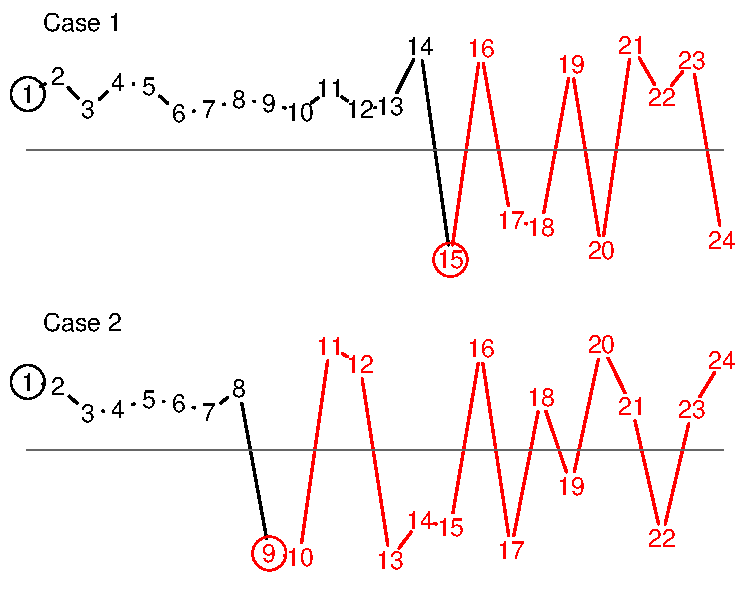
\includegraphics{fig2}
\end{figure}


\section{Case 1, at least as many observations before the first crossing as thereafter}

This is the simplest case. Here, the first $f-1$ observations constitute a run of length $f-1$, and no run in the last $n+f-1$ observations may be longer than that. Therefore, the longest run is $f-1$, and the non-zero probabilities $P_n (C=c,L=l \mid S=1,F=f)$ are confined to the vertical strip $l=f-1$. And, in fact, to only a part of this strip. First, there is at least one crossing, from time $f-1$ to $f$. Also, any further crossings are within the last $n+1-f$ observations, and may be any number between $0$ and $(n+1-f) - 1$. The total number of crossings may therefore be any number between $1$ and $n+1-f$, which means that the non-zero probabilities $P_n (C=c,L=l \mid S=1,F=f)$ are confined to the strip $l=f-1, 1 \leq c \leq n+1-f$. 

The non-zero probabilities $P_n (C=c,L=l \mid S=1,F=f), l=f-1, 1 \leq c \leq n+1-f$ are somehow determined by what happens within the last $n+1-f$ observations. More specifically, the last $n+1-f$ observations constitute a sequence of the same type as the original $n$ observations, only shorter, and with the starting observation fixed on the opposite side of the central line. To put it into a formula, $$P_n (C=c,L=f-1 \mid S=1,F=f)=P_{n+1-f} (C=c-1 \mid S=0)$$ where $C=c-1$ is because the crossing from $f-1$ to $f$ is just before the last $n+1-f$ observations. Similarly, $$P_n (C=c,L=f-1 \mid S=0,F=f)=P_{n+1-f} (C=c-1 \mid S=1)$$ The probabilities on the right hand side of these formulas are for a lower number of observations and are therefore already computed in the iterative procedure. 

Note that the $n+1-f$ observations after the initial run start on opposite side of the centre line. Therefore it is necessary to compute conditional probabilities conditional on starting values both above and below the centre line in the iterative procedure, they cannot be computed separately. The computations are a bit moe complicated in the second case, when the initial run is the shorter part, but the main idea is the same.

\section{Case 2, fewer observations before the first crossing than thereafter}

As in case 1, the total number of crossings is between 1 and $n-f+1$. As to the longest run $L$, it cannot be shorter than $f-1$ or longer than $n-f+1$, and it is necessary to distinguish between values $l=f-1$ and $l \geq f$. A longest run $f-1$ in the entire sequence means that all runs in the last $n-f+1$ observations have length $l \leq f-1$. Therefore $$P_n (C=c,L=f-1 \mid S=1,F=f) = P_{n+1-f} (C=c-1,L \leq f-1 \mid S=0)$$(and similarly conditional on $S=0$). For longer runs, $f \leq l \leq n+1-f$ the longest run has to be within the last $n+1-f$ observations and we have $$P_n (C=c,L=l \mid S=1,F=f) = P_{n+1-f} (C=c-1,L=l \mid S=0)$$(and similarly conditional on $S = 0$). All these conditional probabilies, based on a shorter sequence, have already been computed in an iterative computation procedure.

\section{Simplifications in the symmetric case}

For $p=\frac{1}{2}$ there is a symmetry between crossings up or down, and between success and failure runs. Therefore conditioning on the first observation is not necessary, although it is still necessary to partition on the first crossing $F$. Also, by an induction argument following the iterative procedure, all these probabilities are integer multiples of ${\left( \frac{1}{2} \right)}^{n-1}$ and, in fact, represent a partition of the binomial coefficients in the distribution of $C$, by the values $l=1, \ldots ,n$ of L.  

\section{Precision considerations}

To enhance precision, computations have been performed in the R package \CRANpkg{Rmpfr} \citep{Rmpfr}, an R interface to the GNU MPFR library \citep{FouLHLPZ-2007}. Preliminary investigations pointed to precision problems above values about 50 for sequence length $n$ without this increased precision, but no such problems up to $n=100$ when using \CRANpkg{Rmpfr}. To further enhance precision, probabilities have been multiplied by $m^{n-1}$ where $m$ is a multiplier with default value 2. Thereby very small numbers are avoided, at least to some extent, and the numbers computed are integers in the symmetric case. The joint probabilities for $n=16$ are shown below in this representation:

\tiny{
\strong{
\begin{tabular}{r | r r r r r r r r r r r r r r r r}
\hline
n = 16, p = 0.5&l = 1&2&3&4&5&6&7&8&9&10&11&12&13&14&15&16\\
\hline
c = 0& 0& 0& 0& 0& 0& 0& 0& 0& 0& 0& 0& 0& 0& 0& 0& 1\\
    1& 0& 0& 0& 0& 0& 0& 0& 1& 2& 2& 2& 2& 2& 2& 2& 0\\
    2& 0& 0& 0& 0& 0& 6& 15& 21& 18& 15& 12& 9& 6& 3& 0& 0\\
    3& 0& 0& 0& 1& 34& 90& 106& 84& 60& 40& 24& 12& 4& 0& 0& 0\\
    4& 0& 0& 0& 65& 300& 370& 280& 175& 100& 50& 20& 5& 0& 0& 0& 0\\
    5& 0& 0& 21& 525& 960& 741& 420& 210& 90& 30& 6& 0& 0& 0& 0& 0\\
    6& 0& 0& 266& 1652& 1617& 882& 392& 147& 42& 7& 0& 0& 0& 0& 0& 0\\
    7& 0& 1& 1106& 2716& 1652& 672& 224& 56& 8& 0& 0& 0& 0& 0& 0& 0\\
    8& 0& 36& 2268& 2646& 1080& 324& 72& 9& 0& 0& 0& 0& 0& 0& 0& 0\\
    9& 0& 210& 2640& 1605& 450& 90& 10& 0& 0& 0& 0& 0& 0& 0& 0& 0\\
   10& 0& 462& 1815& 605& 110& 11& 0& 0& 0& 0& 0& 0& 0& 0& 0& 0\\
   11& 0& 495& 726& 132& 12& 0& 0& 0& 0& 0& 0& 0& 0& 0& 0& 0\\
   12& 0& 286& 156& 13& 0& 0& 0& 0& 0& 0& 0& 0& 0& 0& 0& 0\\
   13& 0& 91& 14& 0& 0& 0& 0& 0& 0& 0& 0& 0& 0& 0& 0& 0\\
   14& 0& 15& 0& 0& 0& 0& 0& 0& 0& 0& 0& 0& 0& 0& 0& 0\\
   15& 1& 0& 0& 0& 0& 0& 0& 0& 0& 0& 0& 0& 0& 0& 0& 0\\
\hline
\end{tabular}
}
}

\normalsize

The corresponding joint probabilities are obtained by dividing these integers by $2^{n-1}=2^{15}=32768$, for instance $P(C=5, L=6)=741/32768=0.023$. The highest joint probability is $P(C=7, L=4)=2716/32768=0.083$. It is also seen that a hight proportion of the joint probabilities consists of zeroes, and except for some very small numbers the joint probabilities are concentrated within a narrow sloping band, as also commented in the \CRANpkg{crossrun} vignette, these are fairly general phenomena. For comparison the joint distribution for $n = 16$ is also shown below for $p = 0.6$, a case where observations tend to stay above the midline. These probabilities are still shown in the "times" representation, they are multiplied by $2^{n-1}=32768$, and are shown with one decimal digit:

\tiny{
\strong{
\hspace*{-3em}
\begin{tabular}{r | r r r r r r r r r r r r r r r r}
\hline
n = 16, p = 0.6&l = 1&2&3&4&5&6&7&8&9&10&11&12&13&14&15&16\\
\hline
c = 0&0&0&0&0&0&0&0&0&0&0&0&0&0&0&0&9.3\\
    1&0&0&0&0&0&0&0&0.7&1.6&1.9&2.6&3.8&5.6&8.3&12.4&0\\
    2&0&0&0&0&0&7.5&22.8&41.2&39.3&37.5&35.3&31.9&26.2&16.5&0&0\\
    3&0&0&0&0.7&28.0&88.6&130.0&121.0&102.2&82.8&61.6&38.9&16.6&0&0&0\\
    4&0&0&0&63.4&337.8&485.0&423.3&302.3&202.2&120.6&58.5&18.0&0&0&0&0\\
    5&0&0&15.9&451.3&947.6&845.0&550.2&323.0&166.1&67.6&16.7&0&0&0&0&0\\
    6&0&0&234.2&1619.3&1784.1&1098.1&557.9&245.0&83.5&16.8&0&0&0&0&0&0\\
    7&0&0.7&900.4&2439.2&1660.7&764.3&295.9&87.9&15.2&0&0&0&0&0&0&0\\
    8&0&28.7&1977.6&2518.8&1138.4&386.4&99.8&14.8&0&0&0&0&0&0&0&0\\
    9&0&160.0&2159.1&1427.7&444.0&101.6&13.2&0&0&0&0&0&0&0&0&0\\
   10&0&369.8&1535.6&553.4&118.8&12.8&0&0&0&0&0&0&0&0&0&0\\
   11&0&379.0&582.9&114.6&11.7&0&0&0&0&0&0&0&0&0&0&0\\
   12&0&223.9&127.4&11.5&0&0&0&0&0&0&0&0&0&0&0&0\\
   13&0&68.2&10.9&0&0&0&0&0&0&0&0&0&0&0&0&0\\
   14&0&11.3&0&0&0&0&0&0&0&0&0&0&0&0&0&0\\
   15&0.7&0&0&0&0&0&0&0&0&0&0&0&0&0&0&0\\
\hline
\end{tabular}
}
}
 
\normalsize

\section{Generalization and applications}

The iterative procedure has been generalized to time series where the success probability may vary, as long as the observations are assumed to be independent. This is implemented in a function \code{crossrunchange}. Here, the success probability is replaced by a sequence of probabilities, one for each observation.

The joint distributions for the number of crossings and the longest run may be used to investigate, and possible refine, the Anhoej rules in statistical process control \citep{Anhoej:2014} , Table 1. While these rules have shown to be useful, as seen when preparing \citep{Anhoej:2018} they do not have quite monotone sensitivities and specificities, and preliminary investigations seem to indicate that some improvement is possible. For such work access to the exact joint distributions has decisive advantages compared to simulations. 

\section{Limitations and planned extensions}


There are at present two main limitations. First, in applications in statistical process control when observations are categorized as above or below a midline, the iterative procedure presupposes that the midline is determined from previous data, usually the median. If the midline is the median in the same data set the procedure does not apply. Work is, however, underway to tackle this case. Briefly, the median divides the useful observations (observations not on the median, see \citep{Anhoej:2014} for details) 
into two parts of equal size. The useful observations are then necessarily an even number, say $n=2m$,  the useful observations above the median is a subset of size $m$, and all such subsets are equally probable. To find the number of such subsets for each combination of the number of crossing and the longest run is in fact tractable if it is generalized to all subsets, not necessarily of size $m=n/2$, and an iterative procedure resembling the procedure implemented in \code{crossrunbin} has been developed. The procedure has, due to the large number of such subsets, higher algorithmic complexity in terms of computation time and storage requirements, and it has so far only been possible to use it up to $n=64$.

Preliminary investigations seem to indicate that the difference from the case of a predetermined midline is smaller for longer sequences. A function \code{crossrunem} is planned for inclusion in an update of the package \CRANpkg{crossrun}. 

Another important limitation is that the iterative procedure does not apply for autocorrelated time series. Here also, work is in progress in a simple autocorrelation model in which the probabilities of "success" and "failure" in each observation may depend on the previous observation only, and a function \code{crossrunauto} is planned for inclusion in a future update. The practical value of this procedure is likely to be limited  since decision rules based on the number of crossings and the longest run are probably not particularly useful for autocorrelated series, but at least the procedure may be used to investigate the extent of the problem.

A third limitation is that the code has so far only been checked for $n \leq 100$. In that range it seems to work well. It has been checked with manual computations for $n \leq 6$, and with 100,000 simulations for $n=100$. Specifically, as detailed in the \CRANpkg{crossrun} vignette, the mean and standard deviations for both $C$ and $L$ have been computed, as well as the mean of $C \cdot L$ and also the cumulative distribution functions of $C$ and $L$ separately, with no substantial deviations. It has also been checked for $n \leq 100$ that the marginal distribution of C computed from the joint distribion agrees with the correct binomial distribution in the symmetric case. These last investigations were, in fact, what pointed to the necessity to base the code on \CRANpkg{Rmpfr}. The performance of the procedure has not, however, so far been checked for $n>100$. For applications to statistical process control $n \leq 100$ should be sufficient in most cases, but other applications may require higher $n$.

\section{Conclusions}
 
The \CRANpkg{crossrun} package includes functions for computing the probabilities of the joint distribution of longest run and number of crossings in random data series. To our knowledge, this distribution has not been studied before.
 
The ability to calculate exact probabilities for the joint distribution allows for the development of better prediction limits for longest run and crossings in random data series. In turn, this allows for better separation of signal and noise, i.e. random and non-random variation in statistical process control and possibly also in other areas of application.

\section{Appendix 1: Details on the times representation}

The times representation of the joint distribution is defined as $$\text{Pt}_n ( C=c, L=l \mid S=1 ) = m^{n-1} \cdot P_n ( C=c, L=l \mid S=1 )$$ where $m$ is a multiplier normally set as $m=2$. The case of conditioning on $S=0$, starting below the midline, is similar. Denoting the success probability as $p$ and the failure probability as $q=1-p$ the main decomposition for probabilities is $$P_n ( C=c, L=l \mid S=1) = p^{n-1} \cdot P_n ( C=c, L=l \mid S=1, F=1)+$$

$$ \sum_{f=2}^n p^{f-2} \cdot  q \cdot P_n ( C=c, L=l \mid S=1, F=f)$$
where the first term conditions on $F=1$, by convention corresponding to no crossing, and each of the remaining terms conditions on $F=f, f =2, \ldots , n$ corresponding to the first crossing from $f-1$ to $f$. The corresponding decomposition in the times representation may be written as $$\text{Pt}_n ( C=c, L=l \mid S=1) = (pm)^{n-1} \cdot P_n ( C=c, L=l \mid S=1, F=1) +$$
$$ \sum_{f=2}^n (pm)^{f-2} \cdot  qm \cdot m^{n-f} \cdot P_n ( C=c, L=l \mid S=1, F=f)$$

In the first term for no crossing the probability is simply 1 if $C=0, L=n$ and 0 otherwise. This term is the same in the times representation except for the initial factor in which $p^{n-1}$ is replaced by $(pm)^{n-1}$. In the symmetric case both $pm$ and $qm$ are equal to 1, thus the initial factor is 1 and the term as a whole is actually simpler in the times representation in the symmetric case.

In the remaining terms, for the first crossing from $f-1$ to $f$, there is first a factor $(pm)^{f-2} \cdot  qm$ that is similar to the corresponding factor in the original representation, except that $p$ is replaced by $pm$ and $q$ by $qm$. Again this first factor is actually 1 in the symmetric case. The rest of the term is $m^{n-f} \cdot P_n ( C=c, L=l \mid S=1, F=f)$. As shown previously, the probabilities $P_n ( C=c, L=l \mid S=1, F=f)$ are determined by the joint distribution $P_{n+1-f} ( C=c', L=l' \mid S=0)$ for the observations starting at the end of the first crossing. Here we condition on the opposite starting value $S=0$ since this last part of the sequence starts just where the first crossing has occurred. As to the main part of the term $P_n ( C=c, L=l \mid S=1, F=f)$ we more specifically have seen that it is determined by the joint distribution $P_{n+1-f} ( C=c', L=l' \mid S=0)$ by simple operations in terms of additions and reshuffling only. The corresponding joint distribution in the times representation is $$\text{Pt}_{n+1-f} ( C=c', L=l' \mid S=0)=m^{(n+1-f)-1} \cdot P_{n+1-f} ( C=c', L=l' \mid S=0)$$ where the leading factor $m^{(n+1-f)-1}=m^{n-f}$ is exactly the same as the leading factor in $m^{n-f} \cdot P_n ( C=c, L=l \mid S=1, F=f)$. Therefore the term $$m^{n-f} \cdot P_n ( C=c, L=l \mid S=1, F=f)$$ is determined by the joint distribution $$\text{Pt}_{n+1-f} ( C=c', L=l' \mid S=0)$$ on the times scale by exactly the same additions and reshufflings as apply on the original probability scale.


\section{Appendix 2: R code for the iteration procedure}

The iterative procedure is coded in the function crossrunbin. 

\begin{example}
crossrunbin <- function(nmax   = 100, 
                        prob   = 0.5, 
                        mult   = 2, 
                        prec   = 120, 
                        printn = FALSE) {
  nill   <- mpfr(0, prec)
  one    <- mpfr(1, prec)
  multm  <- mpfr(mult, prec)
  pm     <- mpfr(prob, prec)
  qm     <- one - pm
  pmultm <- pm * multm
  qmultm <- qm * multm
  
  # conditioning of S = first value, pat: above 0, pbt: below 0
  # suffix t: probabilities times multm^(n - 1). 
  # n = 1:
  
  pat <- list(pt1=mpfr2array(one, dim = c(1, 1)))
  pbt <- list(pt1=mpfr2array(one, dim = c(1, 1)))
  pt  <- list(pt1=mpfr2array(one, dim = c(1, 1))) 
  qat <- list(pt1=mpfr2array(one, dim = c(1, 1))) 
  qbt <- list(pt1=mpfr2array(one, dim = c(1, 1)))
  qt  <- list(pt1=mpfr2array(one, dim = c(1, 1)))
  
  for (nn in 2:nmax) {
    pat[[nn]]           <- mpfr2array(rep(nill,nn*nn), dim=c(nn,nn))
    pbt[[nn]]           <- mpfr2array(rep(nill,nn*nn), dim=c(nn,nn))
    rownames(pat[[nn]]) <- c(0:(nn-1))
    rownames(pbt[[nn]]) <- c(0:(nn-1))
    colnames(pat[[nn]]) <- c(1:nn)
    colnames(pbt[[nn]]) <- c(1:nn)
    pat[[nn]][1, nn]     <- (pmultm^(nn-1)) # from cond on no crossing
    pbt[[nn]][1, nn]     <- (qmultm^(nn-1)) # from cond on no crossing

    for (ff in 2:nn) { # from cond on first crossing at ff
      if (nn - ff + 1 <= ff - 1) { # if last part shortest:
        f1 <- ff # unnecessary, but makes code checking easier
        pat[[nn]][2:(nn - f1 + 2), f1 - 1] <- 
          pat[[nn]][2:(nn - f1 + 2), f1 - 1] +
            (pmultm^(f1-2)) * qmultm * 
              qbt[[nn - f1 + 1]][1:(nn - f1 + 1), nn - f1 + 1]
        pbt[[nn]][2:(nn - f1 + 2), f1 - 1] <-
          pbt[[nn]][2:(nn - f1 + 2), f1 - 1] +
            (qmultm^(f1 - 2)) * pmultm * 
              qat[[nn - f1 + 1]][1:(nn - f1 + 1), nn - f1 + 1]
      } # end if last part shortest

      if (nn - ff + 1 > ff - 1) { # if last part longest
        f2 <- ff # unnecessary, but makes code checking easier
        pat[[nn]][2:(nn - f2 + 2), f2 - 1] <- 
          pat[[nn]][2:(nn - f2 + 2), f2 - 1] +
            (pmultm^(f2 - 2)) * 
              qmultm * 
                qbt[[nn - f2 + 1]][1:(nn - f2 + 1), f2 - 1]
        pat[[nn]][2:(nn - f2 + 2), f2:(nn - f2 + 1)] <-
          pat[[nn]][2:(nn - f2 + 2), f2:(nn - f2 + 1)] +
            (pmultm^(f2 - 2)) * 
              qmultm * 
                pbt[[nn - f2 + 1]][1:(nn - f2 + 1), f2:(nn - f2 + 1)]
        pbt[[nn]][2:(nn - f2 + 2), f2 - 1] <-
          pbt[[nn]][2:(nn - f2 + 2), f2 - 1] +
            (qmultm^(f2 - 2)) * 
              pmultm * qat[[nn - f2 + 1]][1:(nn - f2 + 1), f2 - 1]
        pbt[[nn]][2:(nn - f2 + 2), f2:(nn - f2 + 1)] <-
          pbt[[nn]][2:(nn - f2 + 2), f2:(nn - f2 + 1)] +
            (qmultm^(f2 - 2)) * 
              pmultm * 
                pat[[nn - f2 + 1]][1:(nn - f2 + 1),f2:(nn - f2 + 1)]
      } # end if last part longest
    } # end for ff
    
    pt[[nn]]            <- pm * pat[[nn]] + qm * pbt[[nn]]
    qat[[nn]]           <- cumsumm(pat[[nn]])
    qbt[[nn]]           <- cumsumm(pbt[[nn]])
    qt[[nn]]            <- pm*qat[[nn]] + qm*qbt[[nn]]
    rownames(pt[[nn]])  <- c(0:(nn - 1))
    colnames(pt[[nn]])  <- c(1:nn)
    rownames(qat[[nn]]) <- c(0:(nn - 1))
    colnames(qat[[nn]]) <- c(1:nn)
    rownames(qbt[[nn]]) <- c(0:(nn - 1))
    rownames(qat[[nn]]) <- c(0:(nn - 1))
    colnames(qt[[nn]])  <- c(1:nn)
    colnames(qt[[nn]])  <- c(1:nn)

    if (printn) {
      print(nn)
      print(Sys.time())
    } # end optional timing information
  } # end for nn

  names(pat) <-paste("pat", 1:nmax, sep="")
  names(pbt) <-paste("pbt", 1:nmax, sep="")
  names(pt)  <-paste("pt",  1:nmax, sep="")
  names(qat) <-paste("qat", 1:nmax, sep="")
  names(qbt) <-paste("qbt", 1:nmax, sep="")
  names(qt)  <-paste("qt",  1:nmax, sep="")

  return(list(pat = pat, pbt = pbt, pt = pt, qat = qat, qbt = qbt, qt = qt))
} # end function crossrunbin
\end{example}


\section{Appendix 3: Detailed computation, illustrated for n = 7}

We take as an example $n=7$ in the symmetric case. The joint distributions for $n=1, \ldots, 6$ are taken for granted throughout, since this is an illustration of step 7 in the sequential computation procedure. Then $$P_7 (C=c, L=l \mid S=1) = (0.5)^6 \cdot   P_7 (C=c, L=l \mid S=1,F=1) +    $$  $$(0.5) \cdot P_7 (C=c, L=l \mid S=1,F=2) + (0.5)^2 \cdot P_7 (C=c, L=l \mid S=1,F=3) + \ldots  +$$ $$(0.5)^6 \cdot P_7 (C=c, L=l \mid S=1,F=7) $$
In the times representation these probabilities are multiplied by $2^6$. 

In the contribution from $F=1$ , $P_7 (C=c, L=l \mid S=1,F=1)$ is 1 if $C=0$ and $L=7$ and 0 elsewhere, since $F=1$ is defined as no crossing. This contribution from this first term, in the times representation, is a $7 \times 7$ matrix with a 1 in the upper right corner and zeroes elsewhere. 

In the remaining terms for $f=2, \ldots, 7$ there is a distinction between case 1 when the initial run of $f-1$ observations is at least as long as the rest, and case 2 when this is not the case. For $n=7$, case 1 corresponds to $f=5,6,7$, and case 2 corresponds to $f=2,3,4$. 

In case 1 we start with $f=7$. Then the first 6 observations are above the midline and the last observation is below. This means that $C=1$ and $L=6$. The contribution from this term in the times representation is a matrix with a 1 in the position $(c=1,l=6)$ and zeroes elsewhere. 

The term for $f=6$ is $$(0.5)^5 \cdot   P_7 (C=c, L=l \mid S=1,F=6)$$

The longest run is the initial one, with $l=5$. There is one crossing from observation 5 to 6. In addition, the last two observations start below the midline and constitute a sequence on its own, with equal probabilities 0.5 for zero and for one crossing. Thus $$P_7 (C=1, L=5 \mid S=1,F=6)=P_7 (C=2, L=5 \mid S=1,F=6)=0.5$$
The $0.5$ here gives $(0.5)^6$ when multiplied by the initial factor $(0.5)^5$ in the term. Thus in the times representation this contribution is a matrix with ones at positions $(c=1,l=5)$ and $(c=2,l=5)$ and zeroes elsewhere. 

The term for $f=5$ is $$(0.5)^4 \cdot   P_7 (C=c, L=l \mid S=1,F=5)$$

The longest run is the initial one, with $l=4$. There is one crossing from observation 4 to 5. In addition, the last 3 observations start below the midline and constitute a sequence on its own. The joint distribution of $C$ and $L$ in this sequence is 

\begin{tabular}{l | l l l l}
\hline
n=3&l=1&l=2&l=3\\
\hline
c= 0& 0& 0& 1\\
c= 1& 0& 2& 0\\
c= 2& 1& 0& 0\\
\hline
\end{tabular}

From this we get the marginal distribution for the number of crossings in this last 3 observations in the times representation:

\begin{tabular}{l | l l l l}
\hline
n=3&c=0&c=1&c=2\\
\hline
& 1& 2& 1\\
\hline
\end{tabular}


The number of crossings in the entire sequence is one more, thus these three numbers are placed at positions $(c=1,l=4), (c=2,l=4)$ and $(c=3,l=4)$, respectively. In the original representation these numbers are multiplied by $(0.5)^2$ which together with the initial factor $(0.5)^4$ gives $(0.5)^6$, therefore this matrix is the contribution from this term in the times representation of the entire sequence.

The remaining terms are in case 2 when the initial run is no longer than the rest. Continuing downwards the contribution from $f=4$ is 

$$(0.5)^3 \cdot   P_7 (C=c, L=l \mid S=1,F=4)$$

Now, the initial run of $f-1=3$ observations may or may not be a longest run. To further investigate this we have to look at the joint distribution of the remaining 4 observations whose times representation is 

\begin{tabular}{l | l l l l l}
\hline
n=4&l=1&l=2&l=3&l=4\\
\hline
c= 0& 0& 0& 0& 1\\
c= 1& 0& 1& 2& 0\\
c= 2& 0& 3& 0& 0\\
c= 3& 1& 0& 0& 0\\
\hline
\end{tabular}

The initial run is a longest run if and only of $l \leq 3$ in the last 4 observations:

\begin{tabular}{l | l l}
\hline
n=4&$l \leq 3$&l=4\\
\hline
c= 0& 0& 1\\
c= 1& 3& 0\\
c= 2& 3& 0\\
c= 3& 1& 0\\
\hline
\end{tabular}

In the joint distribution for the entire sequence, $l$ is therefore 3 or 4, and the contribution to the joint distribution of $C$ and $L$ for the entire sequence is given by the table above, only with one more crossing:

\begin{tabular}{l | l l l l l l l}
\hline
n=7&l=1&l=2&l=3&l=4&l=5&l=6&l=7\\
\hline
c= 0& 0& 0& 0& 0& 0& 0& 0\\
c= 1& 0& 0& 0& 1& 0& 0& 0\\
c= 2& 0& 0& 3& 0& 0& 0& 0\\
c= 3& 0& 0& 3& 0& 0& 0& 0\\
c= 4& 0& 0& 1& 0& 0& 0& 0\\
c= 5& 0& 0& 0& 0& 0& 0& 0\\
c= 6& 0& 0& 0& 0& 0& 0& 0\\
c= 7& 0& 0& 0& 0& 0& 0& 0\\
\hline
\end{tabular}


Continuing with $f=3$, the term is $$(0.5)^2 \cdot   P_7 (C=c, L=l \mid S=1,F=4)$$

The initial run of $f-1=2$ observations may or may not be a longest run. The joint distribution for the last 5 observations in the times representation is 

\begin{tabular}{l | l l l l l}
\hline
n=5&l=1&l=2&l=3&l=4&l=5\\
\hline
c= 0& 0& 0& 0& 0& 1\\
c= 1& 0& 0& 2& 2& 0\\
c= 2& 0& 3& 3& 0& 0\\
c= 3& 0& 4& 0& 0& 0\\
c= 4& 1& 0& 0& 0& 0\\
\hline
\end{tabular}

The initial run of 2 observations is a longest run if and only if $l \leq 2$ in the last 5 observations, given by the following table:

\begin{tabular}{l | l l l l}
\hline
n=7&$l \leq 2$&l=3&l=4&l=5\\
\hline
c= 0& 0& 0& 0& 1\\
c= 1& 0& 2& 2& 0\\
c= 2& 3& 3& 0& 0\\
c= 3& 4& 0& 0& 0\\
c= 4& 1& 0& 0& 0\\
\hline
\end{tabular}

The corresponding contribution to the joint distribution for the entire sequence includes these numbers, just that the number of crossings in the entire sequence is one more:

\begin{tabular}{l | l l l l l l l}
\hline
n=7&l=1&l=2&l=3&l=4&l=5&l=6&l=7\\
\hline
c= 0& 0& 0& 0& 0& 0& 0& 0\\
c= 1& 0& 0& 0& 0& 1& 0& 0\\
c= 2& 0& 0& 2& 2& 0& 0& 0\\
c= 3& 0& 3& 3& 0& 0& 0& 0\\
c= 4& 0& 4& 0& 0& 0& 0& 0\\
c= 5& 0& 1& 0& 0& 0& 0& 0\\
c= 6& 0& 0& 0& 0& 0& 0& 0\\
\hline
\end{tabular}


Finally, $f=2$. Then there is a crossing from observation 1 to observation 2. The joint distribution of $C$ and $L$ in the last 6 observations is:

\begin{tabular}{l | l l l l l l}
\hline
n=6&l=1&l=2&l=3&l=4&l=5&l=6\\
\hline
c= 0& 0& 0& 0& 0& 0& 1\\
c= 1& 0& 0& 1& 2& 2& 0\\
c= 2& 0& 1& 6& 3& 0& 0\\
c= 3& 0& 6& 4& 0& 0& 0\\
c= 4& 0& 5& 0& 0& 0& 0\\
c= 5& 1& 0& 0& 0& 0& 0\\
\hline
\end{tabular}

The first "run" of just 1 observation is longest if there are all crossings in the last 6 observations, so this is also the contribution to the joint distribution for the entire sequence, just with one crossing more: 

\begin{tabular}{l | l l l l l l l}
\hline
n=7&l=1&l=2&l=3&l=4&l=5&l=6&l=7\\
\hline
c= 0& 0& 0& 0& 0& 0& 0& 0\\
c= 1& 0& 0& 0& 0& 0& 1& 0\\
c= 2& 0& 0& 1& 2& 2& 0& 0\\
c= 3& 0& 1& 6& 3& 0& 0& 0\\
c= 4& 0& 6& 4& 0& 0& 0& 0\\
c= 5& 0& 5& 0& 0& 0& 0& 0\\
c= 6& 1& 0& 0& 0& 0& 0& 0\\
\hline
\end{tabular}

Adding all contributions we get


\tiny{
\begin{tabular}{l | l l l l l l l}
\hline
n=7,f=1&l=1&l=2&l=3&l=4&l=5&l=6&l=7\\
\hline
c= 0& 0& 0& 0& 0& 0& 0& 1\\
c= 1& 0& 0& 0& 0& 0& 0& 0\\
c= 2& 0& 0& 0& 0& 0& 0& 0\\
c= 3& 0& 0& 0& 0& 0& 0& 0\\
c= 4& 0& 0& 0& 0& 0& 0& 0\\
c= 5& 0& 0& 0& 0& 0& 0& 0\\
c= 6& 0& 0& 0& 0& 0& 0& 0\\
\hline
\end{tabular}
+
\begin{tabular}{l | l l l l l l l}
\hline
n=7,f=2&l=1&l=2&l=3&l=4&l=5&l=6&l=7\\
\hline
c= 0& 0& 0& 0& 0& 0& 0& 0\\
c= 1& 0& 0& 0& 0& 0& 1& 0\\
c= 2& 0& 0& 1& 2& 2& 0& 0\\
c= 3& 0& 1& 6& 3& 0& 0& 0\\
c= 4& 0& 6& 4& 0& 0& 0& 0\\
c= 5& 0& 5& 0& 0& 0& 0& 0\\
c= 6& 1& 0& 0& 0& 0& 0& 0\\
\hline
\end{tabular}
+

\begin{tabular}{l | l l l l l l l}
\hline
n=7,f=3&l=1&l=2&l=3&l=4&l=5&l=6&l=7\\
\hline
c= 0& 0& 0& 0& 0& 0& 0& 0\\
c= 1& 0& 0& 0& 0& 1& 0& 0\\
c= 2& 0& 0& 2& 2& 0& 0& 0\\
c= 3& 0& 3& 3& 0& 0& 0& 0\\
c= 4& 0& 4& 0& 0& 0& 0& 0\\
c= 5& 0& 1& 0& 0& 0& 0& 0\\
c= 6& 0& 0& 0& 0& 0& 0& 0\\
\hline
\end{tabular}
+
\begin{tabular}{l | l l l l l l l}
\hline
n=7,f=4&l=1&l=2&l=3&l=4&l=5&l=6&l=7\\
\hline
c= 0& 0& 0& 0& 0& 0& 0& 0\\
c= 1& 0& 0& 0& 1& 0& 0& 0\\
c= 2& 0& 0& 3& 0& 0& 0& 0\\
c= 3& 0& 0& 3& 0& 0& 0& 0\\
c= 4& 0& 0& 1& 0& 0& 0& 0\\
c= 5& 0& 0& 0& 0& 0& 0& 0\\
c= 6& 0& 0& 0& 0& 0& 0& 0\\
\hline
\end{tabular}
+

\begin{tabular}{l | l l l l l l l}
\hline
n=7,f=5&l=1&l=2&l=3&l=4&l=5&l=6&l=7\\
\hline
c= 0& 0& 0& 0& 0& 0& 0& 0\\
c= 1& 0& 0& 0& 1& 0& 0& 0\\
c= 2& 0& 0& 0& 2& 0& 0& 0\\
c= 3& 0& 0& 0& 1& 0& 0& 0\\
c= 4& 0& 0& 0& 0& 0& 0& 0\\
c= 5& 0& 0& 0& 0& 0& 0& 0\\
c= 6& 0& 0& 0& 0& 0& 0& 0\\
\hline
\end{tabular}
+
\begin{tabular}{l | l l l l l l l}
\hline
n=7,f=6&l=1&l=2&l=3&l=4&l=5&l=6&l=7\\
\hline
c= 0& 0& 0& 0& 0& 0& 0& 0\\
c= 1& 0& 0& 0& 0& 1& 0& 0\\
c= 2& 0& 0& 0& 0& 1& 0& 0\\
c= 3& 0& 0& 0& 0& 0& 0& 0\\
c= 4& 0& 0& 0& 0& 0& 0& 0\\
c= 5& 0& 0& 0& 0& 0& 0& 0\\
c= 6& 0& 0& 0& 0& 0& 0& 0\\
\hline
\end{tabular}
+

\begin{tabular}{l | l l l l l l l}
\hline
n=7,f=7&l=1&l=2&l=3&l=4&l=5&l=6&l=7\\
\hline
c= 0& 0& 0& 0& 0& 0& 0& 0\\
c= 1& 0& 0& 0& 0& 0& 1& 0\\
c= 2& 0& 0& 0& 0& 0& 0& 0\\
c= 3& 0& 0& 0& 0& 0& 0& 0\\
c= 4& 0& 0& 0& 0& 0& 0& 0\\
c= 5& 0& 0& 0& 0& 0& 0& 0\\
c= 6& 0& 0& 0& 0& 0& 0& 0\\
\hline
\end{tabular}
=
\begin{tabular}{l | l l l l l l l}
\hline
n=7&l=1&l=2&l=3&l=4&l=5&l=6&l=7\\
\hline
c= 0& 0& 0& 0& 0& 0& 0& 1\\
c= 1& 0& 0& 0& 2& 2& 2& 0\\
c= 2& 0& 0& 6& 6& 3& 0& 0\\
c= 3& 0& 4& 12& 4& 0& 0& 0\\
c= 4& 0& 10& 5& 0& 0& 0& 0\\

c= 5& 0& 6& 0& 0& 0& 0& 0\\
c= 6& 1& 0& 0& 0& 0& 0& 0\\
\hline
\end{tabular}
}


\normalsize


In these calculations we have tacitly used that the joint distributions are the same whether the sequence starts above or below the midline. This is correct in the symmetric case. In non-symmetric cases it is necessary to distinguish between sequences starting above or below the midline, this is precisely why the computations are somewhat simpler in the symmetric case.

\bibliography{crossrunarticle}




\address{Tore Wentzel-Larsen\\
  Centre for Child and Adolescent Mental Health, Eastern and Southern Norway\\
  Norwegian Centre of Violence and Traumatic Stress Studies \\
  Norway\\
  \email{tore.wentzellarsen@gmail.com}}

\address{Jacob Anh{\o}j\\
  Rigshospitalet, University of Copenhagen\\
  Denmark\\
  (ORCiD  https://orcid.org/0000-0002-7701-1774)\\
  \email{jacob@anhoej.net}}


